% This text is proprietary.
% It's a part of presentation made by myself.
% It may not used commercial.
% The noncommercial use such as private and study is free
% Sep. 2005 
% Author: Sascha Frank 
% University Freiburg 
% www.informatik.uni-freiburg.de/~frank/



\pdfminorversion=5
\pdfobjcompresslevel=3 
\pdfcompresslevel=9

% Full presentation (with overlays, animated bullet items etc)
\documentclass[xcolor={x11names,svgnames,dvipsnames}]{beamer}

% Transparency mode (no overlays)
%\documentclass[xcolor={x11names,svgnames,dvipsnames},trans]{beamer}

% 4-up handout mode
%\documentclass[xcolor={x11names,svgnames,dvipsnames},handout]{beamer}

\usepackage{pgfpages}
\usepackage[vlined]{algorithm2e}
\usepackage[british]{babel}
\usepackage{etex}

%% Glossy pretty look for the presentation and transparency (w/o overlays and animations) versions!
\mode<beamer|trans>{
	\useoutertheme[glossy]{wuerzburg}
	\useinnertheme[shadow,outline]{chamfered}
	\usecolortheme{shark}
}
\setbeamertemplate{navigation symbols}{}
\setbeamertemplate{frametitle continuation}[from second][(cont'd)]
\usefonttheme[stillsansseriftext,stillsansserifsmall]{serif}

%% Save up on ink for the 4-up handouts
\mode<handout>{
	\useoutertheme{wuerzburg}
	\useinnertheme[outline]{chamfered}
	\pgfpagesuselayout{4 on 1}[a4paper, landscape, border shrink=10mm]
	\pgfpageslogicalpageoptions{1}{border code=\pgfstroke}
	\pgfpageslogicalpageoptions{2}{border code=\pgfstroke}
	\pgfpageslogicalpageoptions{3}{border code=\pgfstroke}
	\pgfpageslogicalpageoptions{4}{border code=\pgfstroke}
}

\mode<presentation>{\AtBeginSection{%
		\begin{frame}
			\frametitle{Contents}
			\tableofcontents[currentsection]
		\end{frame}}}
		
		\usepackage{microtype}
		\usepackage[utf8]{inputenc}
		\usepackage[T1]{fontenc}
		\usepackage[osfss]{libertine}
		\usepackage[scaled=.77]{beramono}
		\usepackage{cmap}
		
		\usepackage{relsize,tabularx}
		\usepackage[T1,safe]{tipa}
		\usepackage{dtklogos,hologo,textcomp}
		\usepackage{multicol,booktabs}
		\usepackage{listings}
		\lstset{upquote,keepspaces=true,columns=spaceflexible,
			basicstyle=\ttfamily\scriptsize,%
			breaklines=true,breakindent=0pt,xleftmargin=0pt, xrightmargin=6pt,%
			language=[LaTeX]TeX, texcsstyle=*\bfseries\color{Maroon}, commentstyle=\sffamily\itshape\smaller\color{SeaGreen4},
			emphstyle=\bfseries\color{RoyalBlue3},escapechar={:},
			emphstyle={[2]{\bfseries\color{Sienna2}}},
			postbreak=\mbox{{\smaller\color{gray}$\hookrightarrow$}}
		}
		
		\usepackage{tikz}
		\usetikzlibrary{shapes,arrows,positioning,matrix,chains,backgrounds,fit}
		\tikzstyle{startstop} = [rectangle, rounded corners, minimum width=3cm, minimum height=1cm,text centered, draw=black, fill=red!30]
		\tikzstyle{io} = [trapezium, trapezium left angle=70, trapezium right angle=110, minimum width=3cm, minimum height=1cm, text centered, draw=black, fill=blue!30]
		\tikzstyle{process} = [rectangle, minimum width=3cm, minimum height=1cm, text centered, draw=black, fill=orange!30]
		\tikzstyle{decision} = [diamond, minimum width=3cm, minimum height=1cm, text centered, draw=black, fill=green!30]
		\tikzstyle{arrow} = [thick,->,>=stealth]
		
		\usepackage{multicol}
		\usepackage[version=3]{mhchem}
		\usepackage{chemfig}
		\usepackage{linguex,qtree}
		\let\fg\lingfg
		\usepackage{texshade}
		\usepackage[detect-all]{siunitx}
		\usepackage[siunitx]{circuitikz}
		\usepackage{bytefield}
		\usepackage{auto-pst-pdf}
		\usepackage{pstricks,pst-barcode}
		\usepackage{pgfplots}
		\usepackage{pgfgantt}
		\usepackage[skaknew]{chessboard,skak}
		\usepackage{cwpuzzle}
		\usepackage{gchords,guitar}
		\usepackage{spreadtab}
		\usepackage{ccicons}


\setlength\fboxsep{0pt}
\SetTracking{encoding=*}{-39}

\author[\textsc{Jian} Wang]{\textsc{Jian} Wang\\[1ex]%
{\small\url{wangjian790@gmail.com}\\[-.5ex]\url{}}\\
{\small{Financial math Ph.D Candidate}}\\
{\small{Florida State University}}\\
[0.8ex]\copyright\copyright\copyright\copyright} %\ccbyncsa}

\title{Ensemble methods for measuring dynamics of limit order books}
%\titlegraphic{\ccbyncsa}
\date[\textsc{Financial seminar} 2017]{Fall 2017 advanced financial seminar\\ }%

% Include QR code of slides URL for presentation-mode only -- so that audience
%  can snap it and download it on the spot
\mode<beamer>{\titlegraphic{\begin{pspicture}\psbarcode[scalex=.75,scaley=.75]{http://liantze.penguinattack.org/latextypesetting.html\#mosc11-slides}{eclevel=L}{qrcode}\end{pspicture}}}

\hypersetup{%
pdfauthor={Jian Wang}, %% the "author" field from above includes garbage code...
pdfkeywords={HFC,Machine Learning,general}
}
\begin{document}
\begin{frame}
\maketitle
\end{frame}

%\title{Simple Beamer Class}   
%\author{Sascha Frank} 
%\date{\today} 

\frame{\frametitle{Table of contents}\tableofcontents} 

\section{Brief summary}
\begin{frame}
\frametitle{Brief summary}
\begin{itemize}
	\item Our main goal is to use ensemble machine learning methods to predict the limit order book price \alert{cross over} opportunities.  	
	\item Use high frequency data to predict relatively \alert{long time} future price changing trend(eg. 5 seconds later) to prevent illegal actions.
     \item Features selection: choose what kind of data as our independent variables(\alert{choose $x_i$ s}).  
   	\item Compare the f1 score and calculation time  among different machine learning methods, and show that ensemble methods can improve the \alert{predicting performance} significantly. 
   	\item Test the effect of the data sample size to f1 score 	
   	\item Design a simple trading strategy and demonstrate \alert{out of sample} Profit and Loss(PnL)
\end{itemize}
\end{frame}
\section{High frequency trading}
\begin{frame}


\begin{block}{High frequency trading}
High frequency trading is a specialized case of algorithmic trading involving the \alert{frequent turnover} of many \alert{small positions} of a security.
\end{block}

\begin{columns}
\column{2.3in}
\begin{block}{Positive impact}
\begin{itemize}
\item Increased liquidity
\item Narrowing spreads
\item Improve market efficiency
\item Increase fees for Exchanges  
\end{itemize}
\end{block}

\column{2.3in}
\begin{block}{Negative impact }
\begin{itemize}
\item Impact on the institutional investors.
\item Increase volatility (2010 flash crash)
\item Disadvantages to the small Investors(\alert{asymmetric information})
\end{itemize}
\end{block}
\end{columns}

\end{frame}

\begin{frame}

\textbf{\large{HFT Strategies:}}

\begin{columns}
\column{2.4in}
\textbf{Passive: use limit order book}
\begin{block}{Market Making}
\small{Allow the market maker to purchase a company’s securities and,at the same time, the market maker
is also acted as an underwriter of the securities in a secondary public offering. }
\end{block}
\begin{block}{\alert{Statistical Arbitrage}}
\small{Firms and traders looking to make profits from market arbitrage essentially exploit
 the momentary \alert{inconsistencies} in factors such as rates, prices, and other conditions
 between different exchanges or asset classes}
\end{block}
\column{2.5in}
\textbf{Aggressive: use market book}
\begin{block}{Momentum Ignition }
\small{Ignition strategies involve initiating and canceling a number of trades and orders with a certain security in a particular direction, which may ignite a rapid market price movement.}
\end{block}
\begin{block}{ Order anticipate}
\small{Detection trading which confirms
the existence of large institutional buys or sellers in the marketplace and then trade ahead of these
buyers or sellers in anticipation that their large orders will move market prices}
\end{block}

\end{columns}
\end{frame}



\begin{frame}

\textbf{\large{Market Manipulaiton(illegal):}}\\

\vspace{1cm}
According to Dodd-Frank Wall Street Reform and Consumer Protection Act of 2010
(“Dodd-Frank Act”) 
\begin{columns}
\column{2.4in}

\begin{block}{Spoofing}
\small{Bidding or offering with the intent to
cancel the bid or offer before execution. \alert{The line between spoofing and momentum ignition is ambiguous}}
\end{block}

\column{2.5in}
\begin{block}{Front running}
\small{Trading
securities in personal account based on the knowledge of advance knowledge of pending orders
from its customers.\alert{The line between front running and order anticipate is ambiguous}}
\end{block}

\end{columns}

\vspace{1cm}
May be more \alert{safe} to use passive trading strategies in HFT in the future. We pay more attention to statistical arbitrage methods.

\end{frame}

\section{DataSet}
\begin{frame}
\frametitle{Dataset}
\begin{block}{Limit order book data}
The dataset contains limit order book prices of specific stocks from NASDAQ. For each stock, it divided into two major components: the\alert{ message book} and the \alert{order book}.\\
\begin{itemize}
\item Message book: Contains Time, Prices, Volume, Event Type, Direction

\item Order book: Contains price levels, price and volume in each level for every event.  	

\item Sample sizes: AAPL(400391),AMZN(269748),GOOG(147916),INTC(624040),
MSFT(668765)
\item Date: 2012-06-21
\end{itemize}

\end{block} 

\end{frame}

\begin{frame}
\begin{block}{Message Book}
\textbf{AAPL as example:}
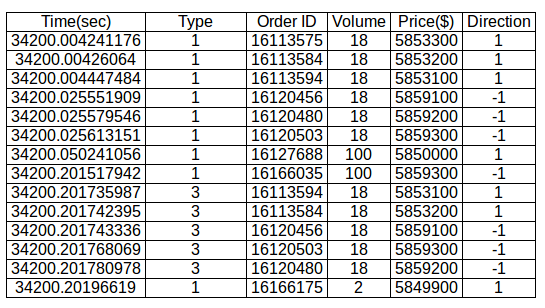
\includegraphics[width=1\textwidth, height=0.6\textheight]{message_book_new.png}
\end{block}

Time is in sec and minimum time change is \alert{nanosecond}, Price is in $10^{-4}$ dollar and each tick is one cent, 5 Event type, such as execution, cancellation and so on, 2 Direction ask and bid. 

\end{frame}

\begin{frame}


\begin{block}{Order book types:}
\begin{table}
\centering
     \begin{tabular}{|c|c|}
     \hline  Type& Description \\ 
     \hline 1& Submission of a new limit order  \\ 
     \hline 2& Cancellation (Partial deletion) \\ 
     \hline 3 & Deletion (Total deletion of a limit order)  \\ 
     \hline 4&   Execution of a visible limit order    \\ 
     \hline 5&   Execution of a hidden limit order\\ 
     \hline 
     \end{tabular} 
\end{table}
\end{block}

\begin{block}{Order book directions:}

\begin{table}
\centering
     \begin{tabular}{|c|c|}
     \hline  Direction& Description \\ 
     \hline -1 &  Sell limit order \\ 
     \hline 1&  Buy limit order\\ 
     \hline
     \end{tabular} 
\end{table}
\end{block}



\end{frame}

\begin{frame}
	\textbf{Order Book:}
	\begin{figure}
		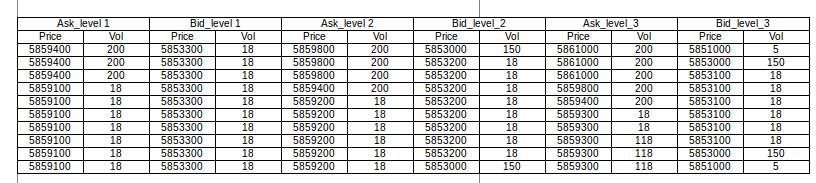
\includegraphics[width=1\textwidth, height=0.5\textheight]{order_book_new.png}
	\end{figure}
From level \alert{1 to level 10}, where the first level is the best bid and ask. Price is in \alert{$10^{-4}$} dollar.	
\end{frame}



\section{Methodology}
\begin{frame}
\frametitle{Methodology}
Six machine learning algorithm candidates:\\
 \vspace{1cm}
Basic methods:logistic regression with L1 penalty, logistic regression with L2 penalty,support vector machine, decision tree method(simply described)\\
\vspace{1cm}
Ensemble methods:Ada-boosting method, random forest method(mainly described).


\end{frame}

\begin{frame}
\frametitle{Methodology}
%
%\setbeamercovered{transparent}
%\begin{block}{Stock Return series}
%\begin{equation}
%R_t = ln( S_{t+1})-ln(S_t)
%\end{equation}
%Where $R_t$ is the stock return at trading day t and $S_t$ is the closing price of stock at trading day t.
%\end{block}
%\setbeamercovered{transparent}
\begin{block}{Logistic regression}
\begin{center}
$ln{\frac{F(x)}{1-F(x)}}=\beta_0+\sum_i\beta_ix_i$\\
\end{center}
\end{block}

\begin{block}{Ridge regression}
\begin{center}
$\hat{\beta}^{ridge}=argmin_{\beta}\{\sum_{i=1}^p{(y_i-\hat{y_i})^2}+{\color{red}\lambda \sum_{j=1}^p\beta_j^2}\}$
\\
\end{center}
\end{block}

\begin{block}{Lasso regression}
\begin{center}
$\hat{\beta}^{lasso}=argmin_{\beta}\{\sum_{i=1}^p{(y_i-\hat{y_i})^2}+{\color{red}\lambda\sum_{j=1}^p |\beta_j|}\}$\\
\end{center}
\end{block}

\end{frame}


\begin{frame}
\frametitle{Methodology}
Comparison of L1 and L2 Penalized Model \\
\begin{columns}
\column{2.3in}
	\begin{block}{Ridge regression}
$\hat{\beta}^{ridge}=argmin_{\beta}\{\sum_{i=1}^p{(y_i-\hat{y_i})^2}+{\color{red}\lambda \sum_{j=1}^p\beta_j^2}\}$

\end{block}
\textbf{Coefficients}:
 \begin{figure}
     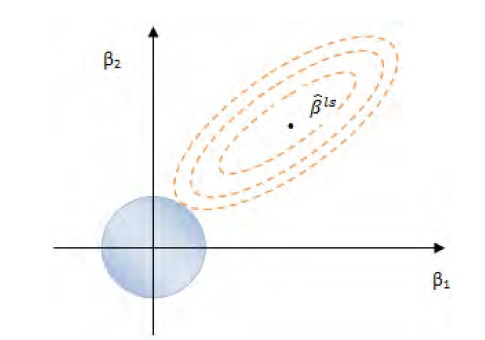
\includegraphics[width=0.9\textwidth, height=0.42\textheight]{ridge.jpg}

    \end{figure}

\column{2.3in}
\begin{block}{Lasso regression}

$\hat{\beta}^{lasso}=argmin_{\beta}\{\sum_{i=1}^p{(y_i-\hat{y_i})^2}+{\color{red}\lambda\sum_{j=1}^p |\beta_j|}\}$

\end{block}

\textbf{Coefficients}:
 \begin{figure}
     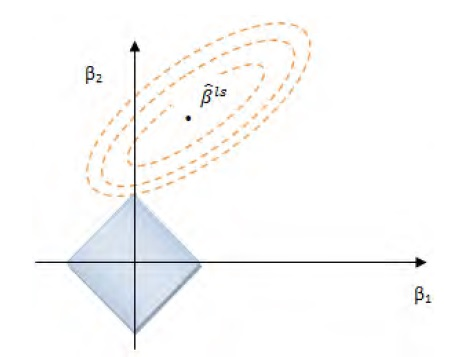
\includegraphics[width=0.9\textwidth, height=0.42\textheight]{lasso.jpg}
    \end{figure}
\end{columns}


\end{frame}

\begin{frame}
\frametitle{Methodology}
Comparison of L1 and L2 Penalized Model \\
\begin{columns}
\column{2.3in}
	\begin{block}{Ridge regression}
$\hat{\beta}^{ridge}=argmin_{\beta}\{\sum_{i=1}^p{(y_i-\hat{y_i})^2}+{\color{red}\lambda \sum_{j=1}^p\beta_j^2}\}$

\end{block}
\textbf{Path:}:
 \begin{figure}
     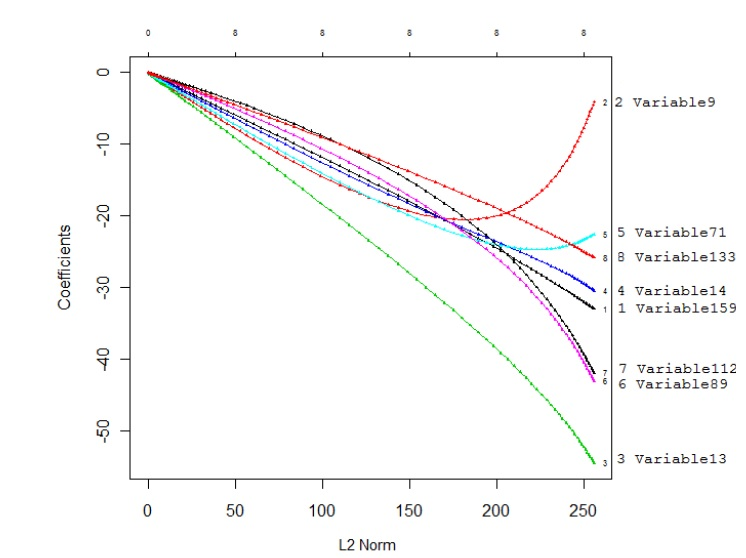
\includegraphics[width=0.8\textwidth, height=0.45\textheight]{ridge_p.jpg}

    \end{figure}

\column{2.3in}

\begin{block}{Lasso regression}

$\hat{\beta}^{lasso}=argmin_{\beta}\{\sum_{i=1}^p{(y_i-\hat{y_i})^2}+{\color{red}\lambda\sum_{j=1}^p |\beta_j|}\}$

\end{block}

\textbf{Path:}:
 \begin{figure}
     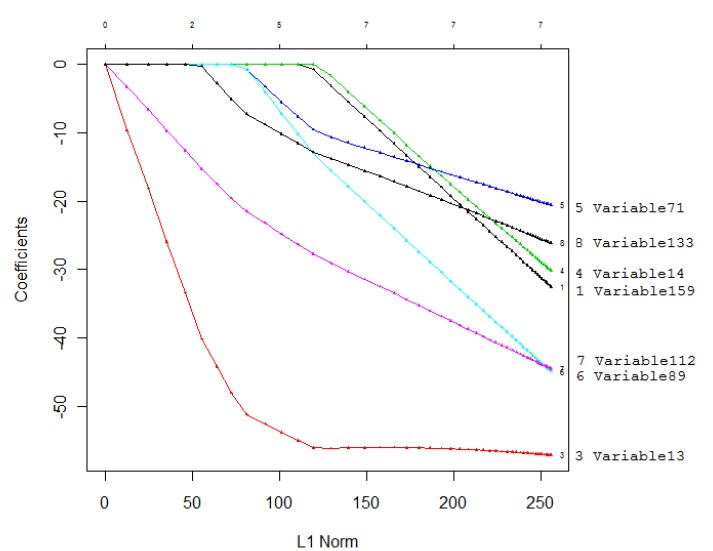
\includegraphics[width=0.8\textwidth, height=0.45\textheight]{lasso_p.jpg}

    \end{figure}
\end{columns}

\end{frame}

\begin{frame}
\frametitle{Methodology}
\begin{block}{Support vector machine}
{\small
• Introduced in COLT-92 by Boser, Guyon \& Vapnik. Became
rather popular since.\\
• Theoretically well motivated algorithm: developed from Statistical
Learning Theory (Vapnik \& Chervonenkis) since the 60s.\\
• Empirically good performance: successful applications in many
fields (bioinformatics, text, image recognition, . . . )\\
}
\end{block}

\begin{columns}<+->
\begin{column}{0.6\textwidth}
\small {
Try to maximize the margin:\\ 
$r=1/||w||,y_j=1,-1$\\
\alert{primal form}:\\
$\max\limits_{W,b}\ r= 1/||W||$\\
$s.t.(W^Tx_j+b)y_j>=1$\\
\alert{Dual form}:\\
$\max\limits_{\alpha_1,...,\alpha_M}\ \sum\alpha_l-\frac{1}{2}\sum_{j=1}^{M}\sum_{k=1}^{M}\alpha_j\alpha_k y_j y_k<X_j,X_k>$\\
s.t.$\alpha_l\geq 0$, $\sum_{l=1}^{M}\alpha_ly_l=0$
}
\end{column}
\begin{column}{.4\textwidth}
     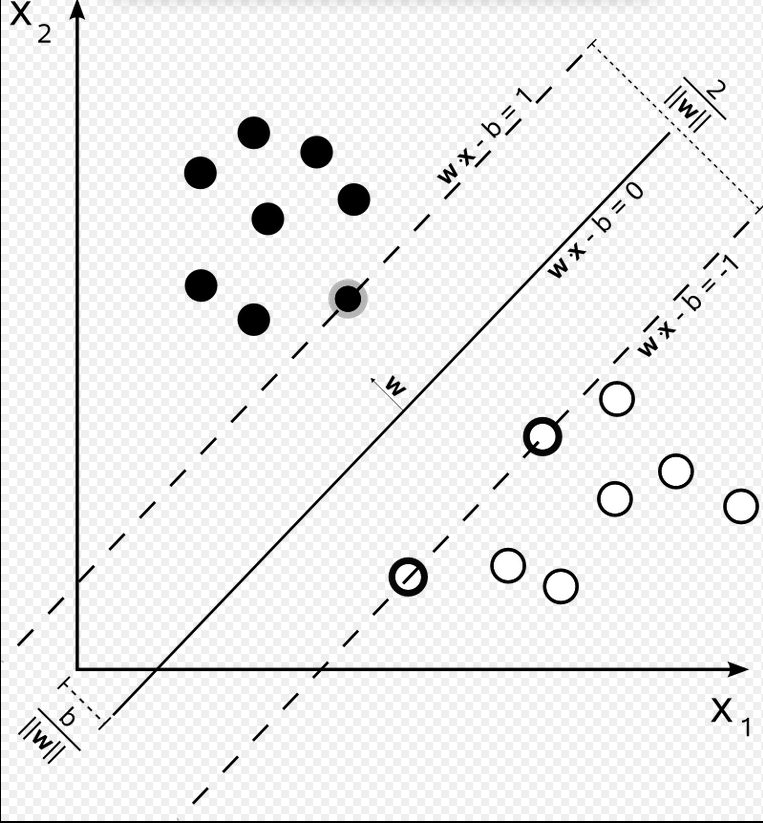
\includegraphics[width=0.8\textwidth, height=0.4\textheight]{svm.png}
\end{column}
\end{columns}
\end{frame}

\begin{frame}
\frametitle{Methodology}
\setbeamercovered{transparent}
\begin{block}{Kernel functions}
To solve non-linearly separable issue, we can use the kernel function to calculate the inner product in high dimensional cases in its original feature spaces.
\end{block}
\begin{block}{Example:two dimension polynomial}
$k(x,z)=(x^Tz)^2$\\
$=(x_1^2,\sqrt{2}x_1x_2,x_2^2)^T(z_1^2,\sqrt{2}z_1z_2,z_2^2)$\\
$=\Phi(x)^T\Phi(z)$\\
\end{block}
\begin{block}{Kernel functions that we used}
\small{
\textbullet\ {Linear kernel:  $k(x,y)=x^Ty+c$}\\
\textbullet\ {Polynomial Kernel:  $k(x,y)=(\alpha x^Ty+c)^d$}\\
\textbullet\ {Radial basis function kernel(RBF):  $k(x,y)=exp(-\gamma||x-y||^2)$}
}
\end{block}
\end{frame}

\begin{frame}
\frametitle{Methodology}
\textbf{Decision tree:}
Use \textbf{entropy and information gain} to define the root and parent nodes, split the data into different classes.\\
\textbf{Example:}
Know the history of playing golf or not, given new data, make prediction\\ 
      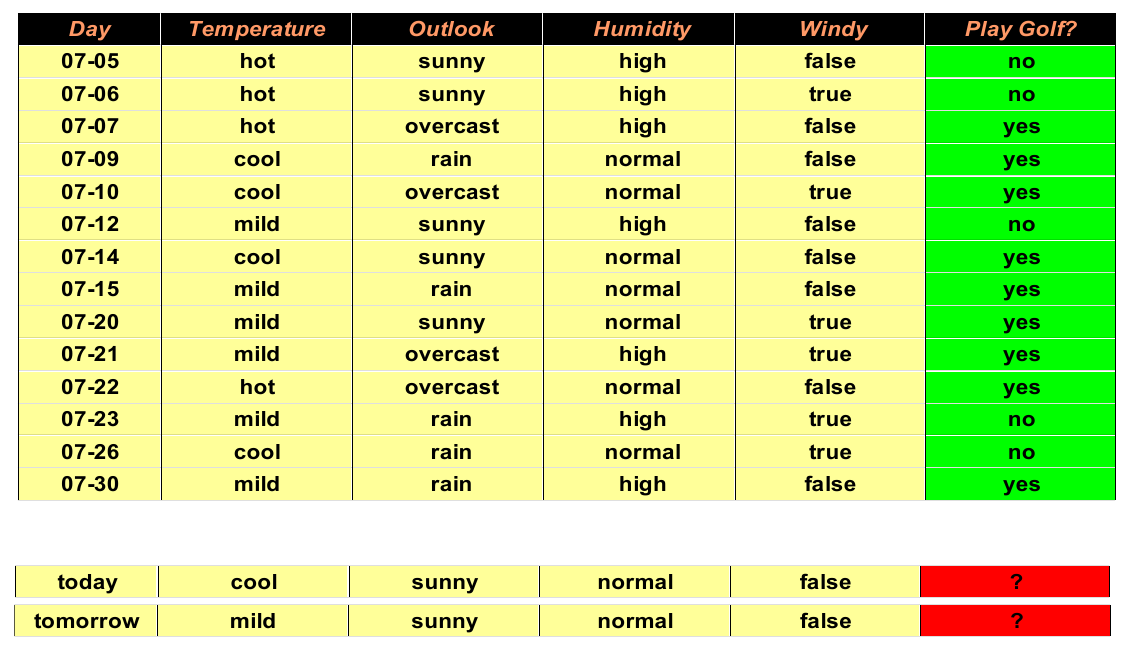
\includegraphics[width=1\textwidth, height=0.7\textheight]{decision_tree1.png}
\end{frame}

\begin{frame}
\frametitle{Methodology}


      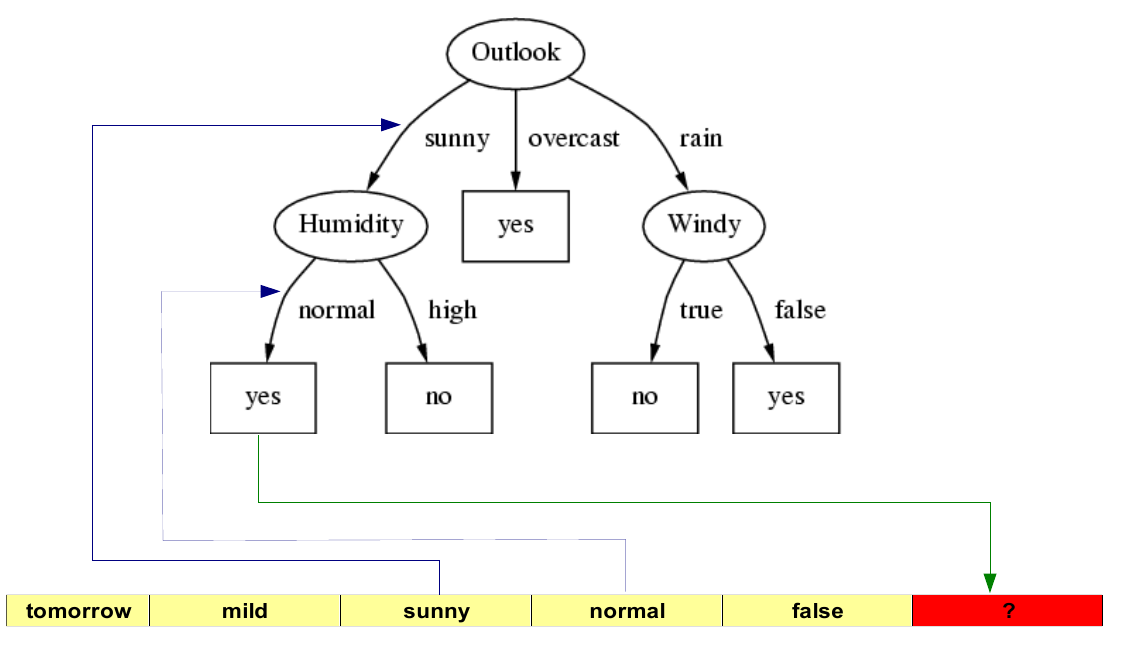
\includegraphics[width=1\textwidth, height=0.7\textheight]{decision_tree2.png}
\end{frame}

\begin{frame}
\frametitle{Methodology}
\textbf{Which attribute to select as the root?}
\vskip 0.5cm
      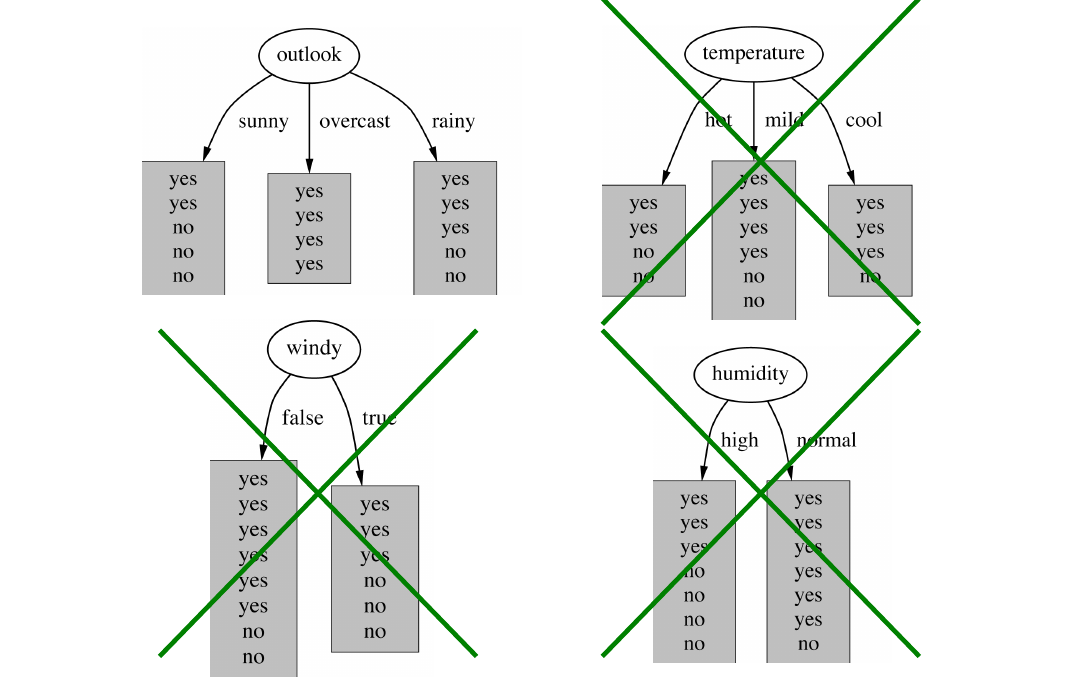
\includegraphics[width=1\textwidth, height=0.7\textheight]{decision_tree3.png}
\end{frame}

\begin{frame}
\frametitle{Methodology}
\begin{block}{Entropy:}
Entropy is a measure for un-orderedness\\
\begin{center}
$E(s)=-\sum_{i=1}^n p_i log_2p_i$
\end{center}
\textcolor{blue}{Outlook = sunny:} 3 examples yes, 2 examples no\\
\begin{center}
$E(outlook=sunny)=-\frac{2}{5}log{\frac{2}{5}}-\frac{3}{5}log{\frac{3}{5}}=0.971$
\end{center}

\textcolor{blue}{Outlook = overcast:}  4 examples yes, 0 examples no\\

\begin{center}
$E(outlook=overcast)=-1log{1}-0log{0}=0$
\end{center}
\textcolor{blue}{Outlook = rainy:} 2 examples yes, 3 examples no:\\
\begin{center}
$E(outlook=sunny)=-\frac{3}{5}log{\frac{3}{5}}-\frac{2}{5}log{\frac{2}{5}}=0.971$
\end{center}
\end{block}

\end{frame}

\begin{frame}
\frametitle{Methodology}
\begin{block}{Information Gain for attribute A:}
When an attribute A splits the set S into subsets $S_i$
\begin{itemize}
\item  we compute the average entropy
\item  and compare the sum to the entropy of the original set S
\end{itemize}
\begin{equation*}
Gain(S,A)=E(S)-I(S,A)=E(S)-\sum_{i}\frac{|S_i|}{|S|}E(S_i)
\end{equation*}

The attribute that maximizes the difference is selected
\end{block}

\end{frame}

\begin{frame}
\frametitle{Methodology}


      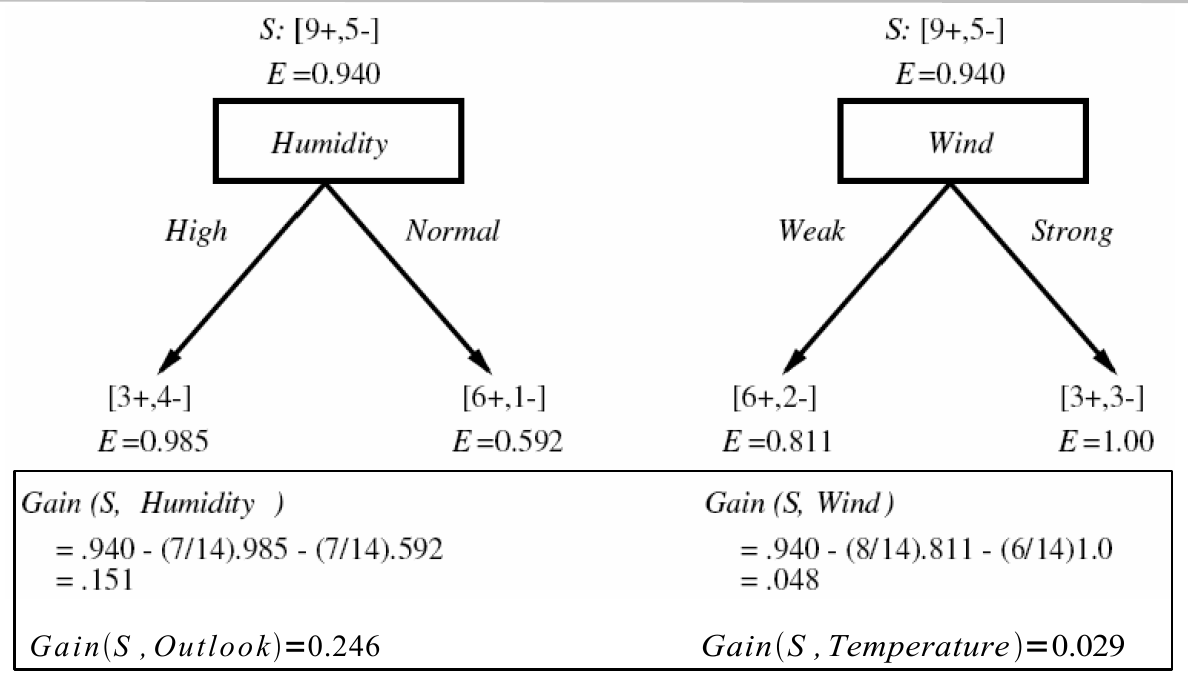
\includegraphics[width=1\textwidth, height=0.7\textheight]{decision_tree4.png}
\end{frame}

\begin{frame}
\frametitle{Methodology}


      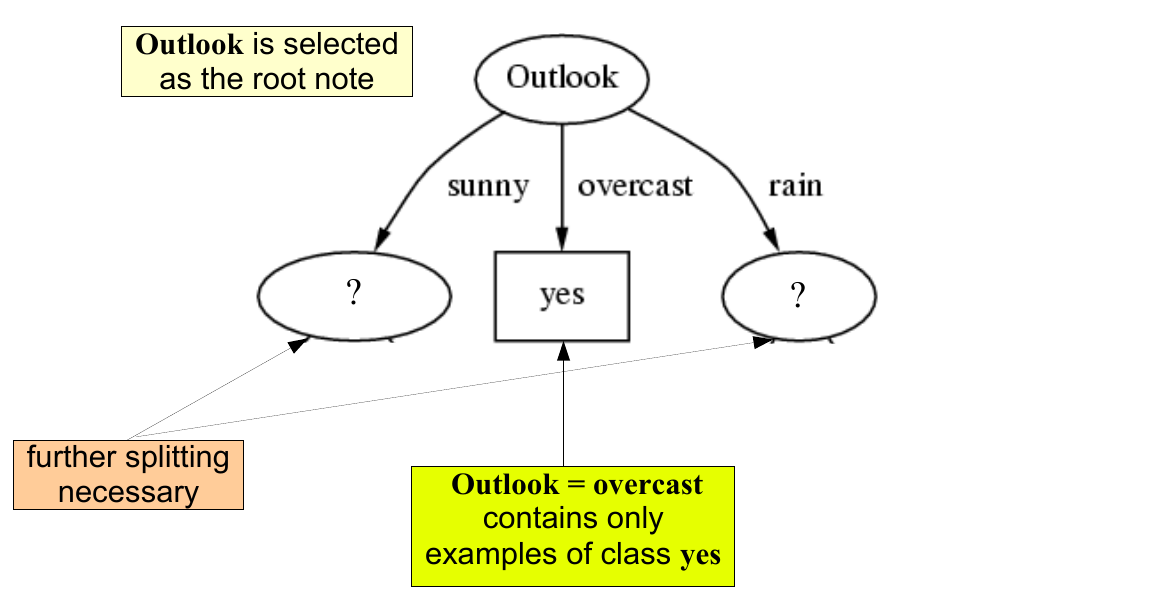
\includegraphics[width=1\textwidth, height=0.7\textheight]{decision_tree5.png}
\end{frame}

\begin{frame}
\frametitle{Methodology}


      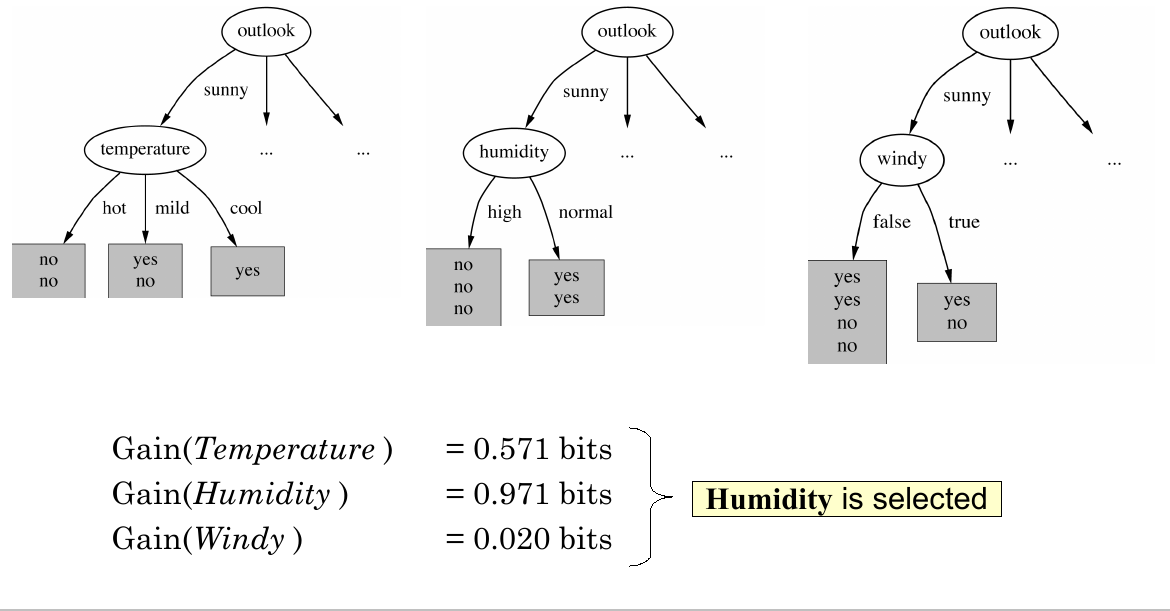
\includegraphics[width=1\textwidth, height=0.7\textheight]{decision_tree6.png}
\end{frame}


\begin{frame}
\frametitle{Methodology}


      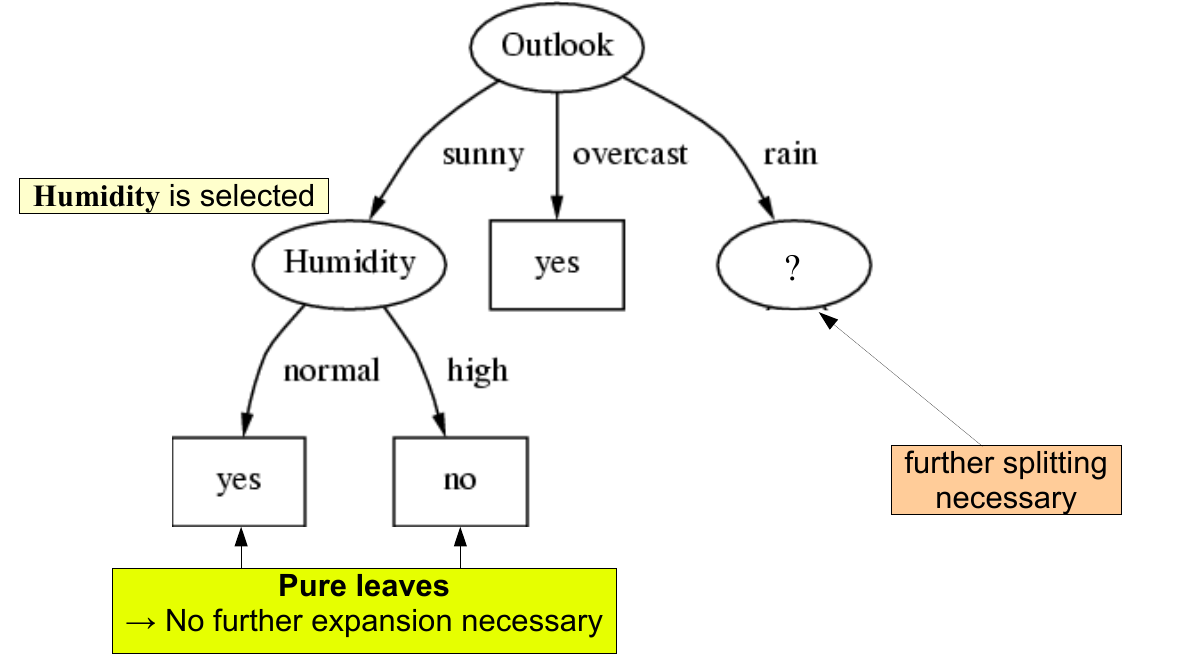
\includegraphics[width=1\textwidth, height=0.7\textheight]{decision_tree7.png}
\end{frame}

\begin{frame}
\frametitle{Methodology}
\textbf{Final structure:}
\vskip 0.3 cm
      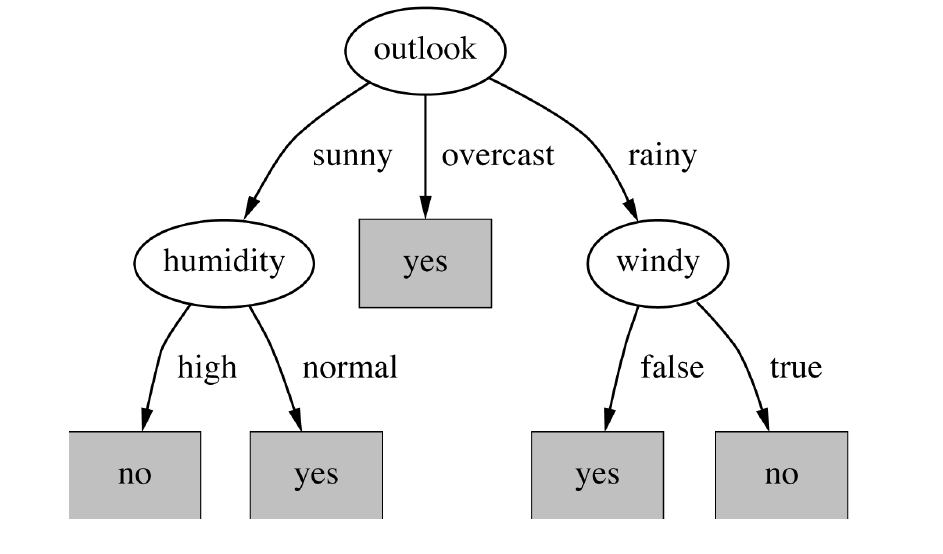
\includegraphics[width=1\textwidth, height=0.7\textheight]{decision_tree8.png}
\end{frame}






\begin{frame}
\frametitle{Methodology}

	\begin{block}{Ensembling methods: the most important part}
		\textbf{IDEA:} 
			 \begin{itemize}
			 \item Do not learn a single class but learn a set of classifiers
			 \item Combine the predictions of multiple classifiers	 
			 \end{itemize}
		\textbf{Motivation:} 
			 \begin{itemize}
			 \item Reduce variance: results are less dependent on peculiarities of
			 a single training set
			 
			 \item Reduce bias: a combination of multiple classifiers may learn a
			 more expressive concept class than a single classifier
			 	 
			 \end{itemize}
		\textbf{ KEY STEP:} 
			 \begin{itemize}
			 \item  Formation of an ensemble of diverse classifiers from a
			 single training set			 
			 \end{itemize}


	\end{block}
\end{frame}



\begin{frame}
\frametitle{Methodology}

	\begin{block}{Why do ensembles work?}
		\textbf{Suppose there are 25 base classifiers:} 
			 \begin{itemize}
			 \item Each classifier has error rate, $\epsilon= 0.35$
			 
			 \item  Assume classifiers are independent
			 			 	 
			 \end{itemize}
		\textbf{Probability that the ensemble classifier makes a wrong
		prediction:} 
			 \begin{itemize}
			 \item The ensemble makes a wrong prediction if the majority of
			 the classifiers makes a wrong prediction
			 
			 
			 \item The probability that 13 or more classifiers err is:
			 \begin{equation*}
				 \sum_{i=13}^{25} {25 \choose i}\epsilon^i(1-\epsilon)^{25-i}\approx 0.06\ll \epsilon
			 \end{equation*}
			 \end{itemize}

	\end{block}
\end{frame}


\begin{frame}
	\frametitle{Methodology}
	\setbeamercovered{transparent}
	\begin{block}{First ensemble method: AdaBoost method}
	  \begin{itemize}
	  \item Introduced in 1990s
	  \item Originally designed for classification problems
	  \item Later extended to regression
	  \item Motivation - a procedure that \alert{combines the outputs of many “weak” classifiers to produce a powerful “committee”}	 
	  \item Put more weight on mis-classification data each time  
	  \end{itemize}
	\end{block}
\end{frame}



\begin{frame}
	\frametitle{Methodology}
	\setbeamercovered{transparent}
	\begin{block}{Boosting methods}
      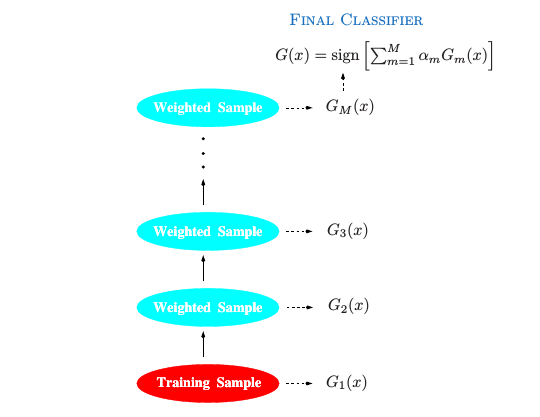
\includegraphics[width=0.8\textwidth, height=0.7\textheight]{boosting.png}
	\end{block}	
\end{frame}


\begin{frame}
	\frametitle{Methodology}
	\begin{block}{AdaBoost example: TOY example:}
      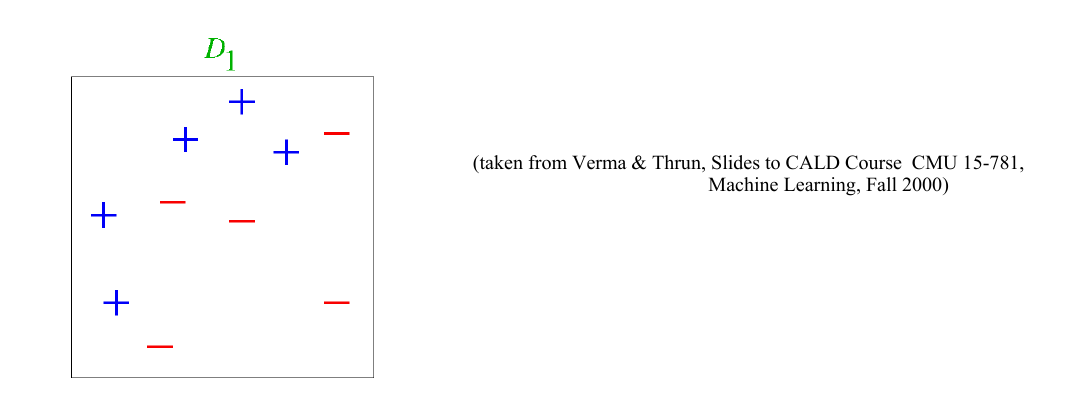
\includegraphics[width=1\textwidth, height=0.5\textheight]{toy_example.png}
	\end{block}	
\end{frame}


\begin{frame}
	\frametitle{Methodology}
   \small{\textbf{Round 1:}}

	\begin{block}{AdaBoost example: TOY example:}

      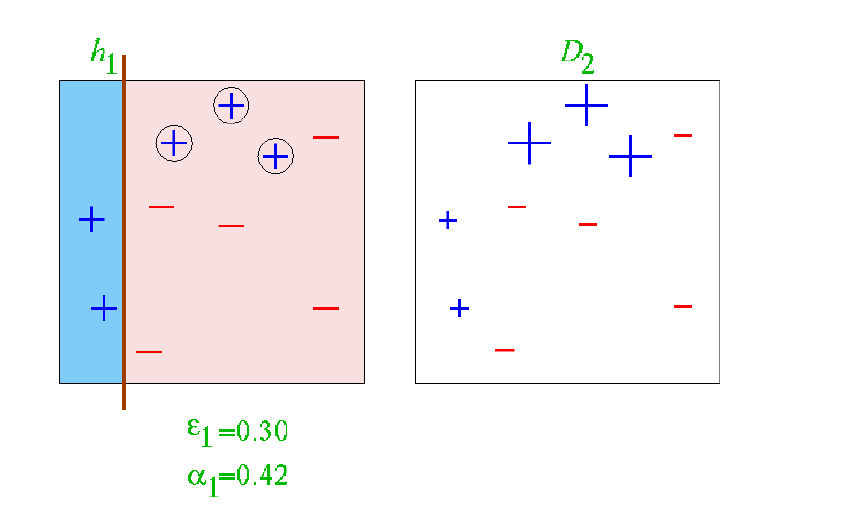
\includegraphics[width=1\textwidth, height=0.6\textheight]{round_1.png}
	\end{block}	
\end{frame}

\begin{frame}
	\frametitle{Methodology}
	\setbeamercovered{transparent}
	 \small{\textbf{Round 2:}}\\
		
	\begin{block}{AdaBoost example: TOY example:}

      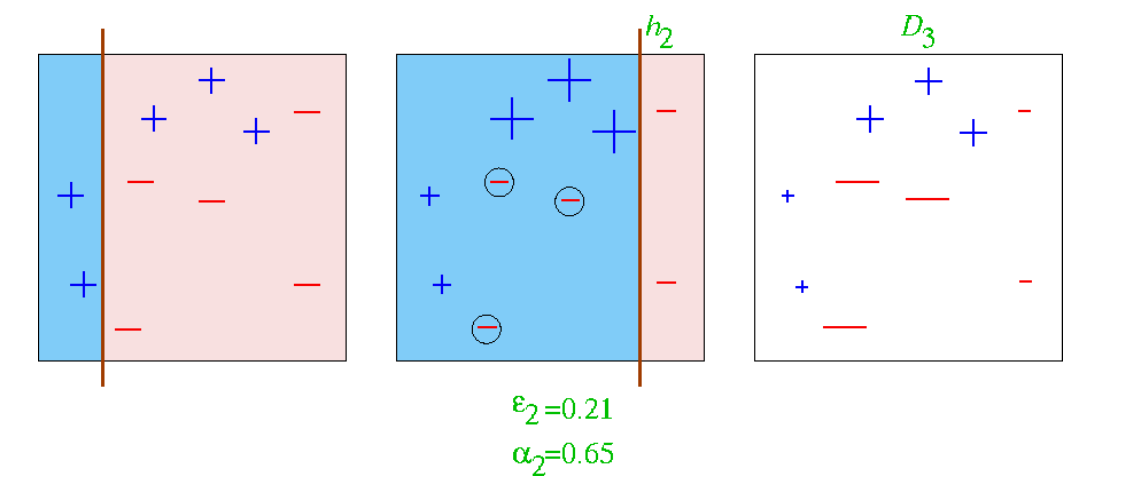
\includegraphics[width=1\textwidth, height=0.6\textheight]{round_2.png}
	\end{block}	
\end{frame}

\begin{frame}
	\frametitle{Methodology}
	\setbeamercovered{transparent}
			\small{\textbf{Round 3:}}\\
			
	\begin{block}{AdaBoost example: TOY example:}

      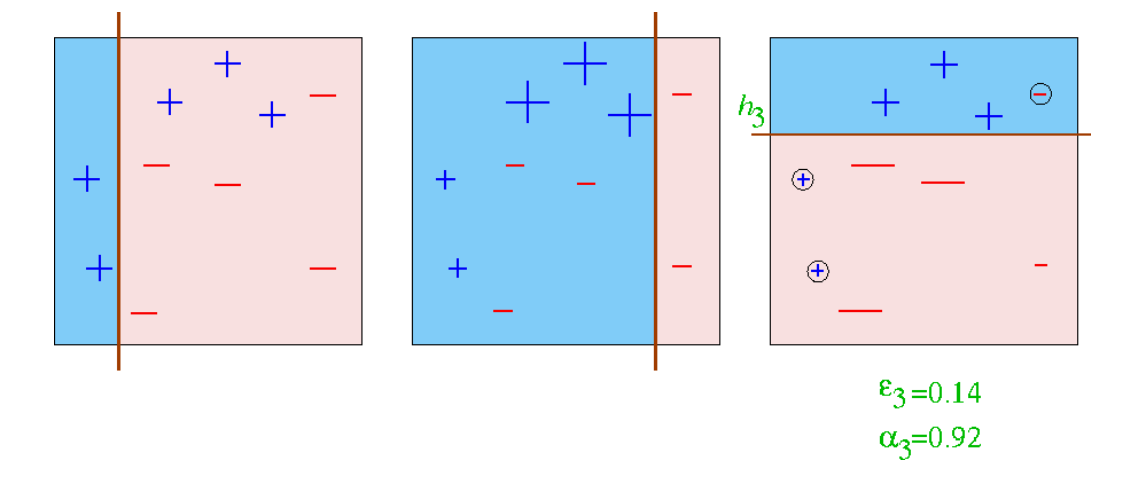
\includegraphics[width=1\textwidth, height=0.6\textheight]{round_3.png}
	\end{block}	
\end{frame}


\begin{frame}
	\frametitle{Methodology}
	\setbeamercovered{transparent}
			\small{\textbf{Final round:}}\\
			
	\begin{block}{AdaBoost example: TOY example:}

      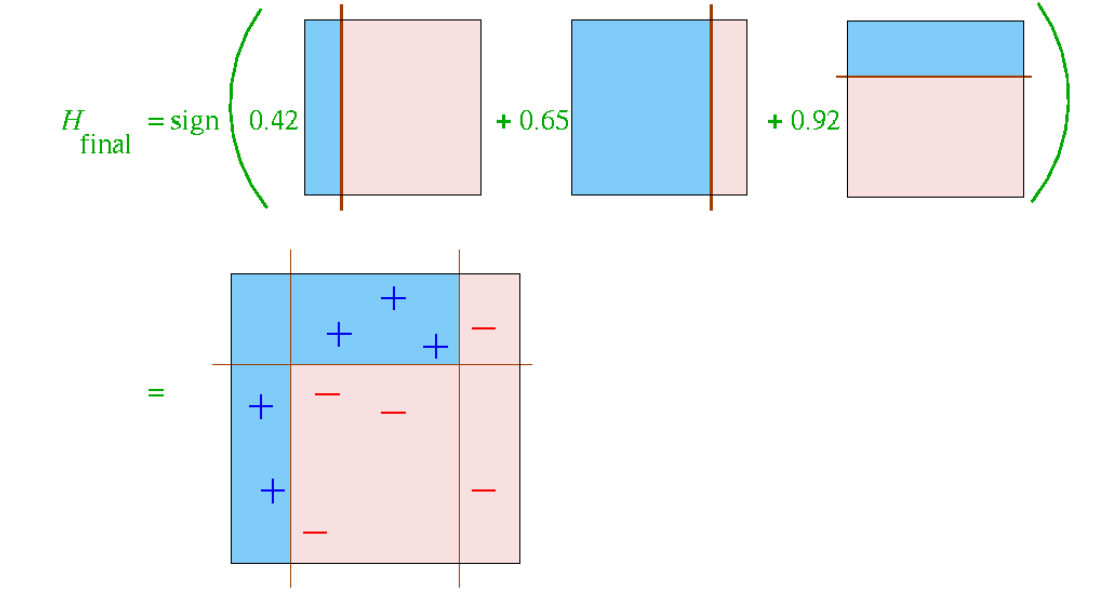
\includegraphics[width=1\textwidth, height=0.6\textheight]{round_4.png}
	\end{block}	
\end{frame}




\begin{frame}
	\frametitle{Methodology}
		\begin{block}{Second ensemble method: Random forest}	
			Dataset: N samples, each having M attributes (features)\\
			A value m<M is chosen,$m \approx \sqrt{M} $ or $m \approx log{M}$\\
		Growing one tree:
		
		\begin{itemize}
		\item Select N samples randomly with replacement (bootstrap)\\
		\item At each node, m attributes are selected randomly from the M
		\item The best binary split from the m attributes (based on
		information gain) is chosen\\
		\item The tree is fully grown, no pruning		
		
		\end{itemize}
		Loop the above process several times. Given an observation:\\
		\begin{itemize}
		\item Each decision tree votes for a class\\
		\item The class with most votes is the final result\\		
		\end{itemize}	 
		\end{block}	
\end{frame}

\begin{frame}
\begin{columns}

	\begin{column}{.5\textwidth}
		\textbf{Adaboosting algorithm:}\\
		\scriptsize {
			\begin{algorithm}[H]
				    \dontprintsemicolon
				    \linesnumbered
				    \nl Initialize the observation weights $\omega_i$=$1/N$,$i$=1,2,...,$N$\;
				    \nl \For{m=1 to M}{
				      Fit a classifer $G_m(x)$ to the training data using weights $\omega_i$\;
				       Compute \\
				      \begin{equation*}
				      err_m=\frac{\sum_{i=1}^{N}\omega_i I(y_i \neq G_m(x_i))}{\sum_{i=1}^{N}\omega_i}
				      \end{equation*}
				     Compute $\alpha_m=log((1-err_m)/err_m)$\;
				     Set $\omega_i \gets \omega_i \cdot exp[\alpha_m \cdot I(y_i \neq G_m(x_i))]$, $i =1,2,...,N$ \;
				    }
				    \nl Output $G(x)=sign[\sum_{m=1}^{M}\alpha_m G_m(x)]$ 
				  \end{algorithm}\\
				  }
		
		\small{\textbf{source:ESL}}\\
		\alert{\textbullet\ Put more weights on the false classification data}\\
		\alert{\textbullet\ Average each classifer based on error to get the strong classifer}\\
		\alert{\textbullet\ Maybe the strongest classifer among the out of box classifers}
	\end{column}
	\begin{column}{.5\textwidth}
		\textbf{Random forest algorithm:}\\
		\scriptsize {
		\begin{algorithm}[H]
				         		    \dontprintsemicolon
				         		    \linesnumbered				         		    
				         		    \nl \For{b=1 to B}{
				         		    {(a) Draw a bootstrap sample $Z^*$ of size N from the training data.\\}
				         		    {(b) Grow a random-forest tree $T_b$ to the bootstrapped data, by re-
				         		    cursively repeating the following steps for each terminal node of
				         		    the tree, until the minimum node size $n_{min}$ is reached.\\
				         		    i. Select m variables at random from the p variables.\\
				         		    ii. Pick the best variable/split-point among the m.\\
				         		    iii. Split the node into two daughter nodes.\\
				         		    
				         		    }				         		    
				         		    }
				         		    \nl Output the ensemble of trees $\{T_b\}_1^B$ \\
				         		    To make a prediction at a new point x:\\
				         		    \nl Let $\hat{C}_b(x)$ be the class prediction of the bth random forest tree. Then $\hat{C}_{rf}^B(x)$= majority vote $\{\hat{C}_b(x)\}_1^{B}$
			\end{algorithm} \\
				         		   }
		
	    \small{\textbf{source:ESL}}\\
	    \alert{\textbullet Combine feature selection and bootstrap methods}\\
	    \alert {\textbullet Correct for decision trees' habit of overfitting to their training set}
	\end{column}
\end{columns}	
\end{frame}

%\begin{frame}
%	\begin{block}{Boosting methods error rate evolution}
%		\footnotesize{
%      Boosting method can dramatically increase the performance of even a very weak classifier.We further implement the figure 10.2 in the ESL for example. Suppose features $X_1, X_2,...,X_10$ are standard independent Gaussian, and the deterministic target $Y$ is defined by:\\
%      \begin{equation*}
%       Y=\left\{
%       \begin{array}{l}
%       1\ \quad\quad if \sum_{j=1}^{10}X_j^2>\chi_{10}^2(0.5) \\
%       -1\ \quad otherwise\\
%       \end{array}
%       \right.    
%      \end{equation*} 
%    where $\chi_{10}^2(0.5)$ is the median of a chi square random variable with 10 degrees of freedom.}
%	\end{block}
%	\begin{columns}		
%		\begin{column}{.6\textwidth}
%			\begin{center}
%						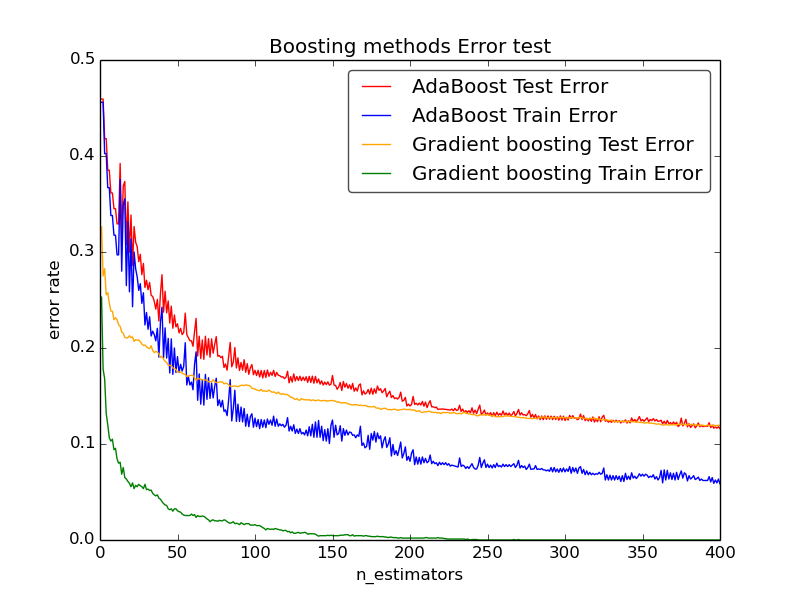
\includegraphics[width=0.8\textwidth, height=0.45\textheight]{boosting_error.png}
%			\end{center}
%		\end{column}
%		\begin{column}{.4\textwidth}
%			\begin{itemize}
%				\small{
%			\item Boosting methods can reduce the prediction error rate to around one third of the original.
%			\item In this case, Gradient boosting method performance better}
%			\end{itemize}
%		\end{column}
%	\end{columns}	
%\end{frame}


\section{Model fit}

\newcommand<>{\hover}[1] {\uncover#2 {
	\begin{tikzpicture}[remember picture,overlay,fill opacity=1]
    \draw [fill opacity=1] (current page.south west)
	rectangle (current page.north east);
	\node at (current page.center) {#1};
	\end{tikzpicture}}
	}

\begin{frame}
\frametitle{Model fit}
\begin{columns}		
		\begin{column}{.5\textwidth}
		   \textbf{order book snapshot:}\\
			\begin{center}
						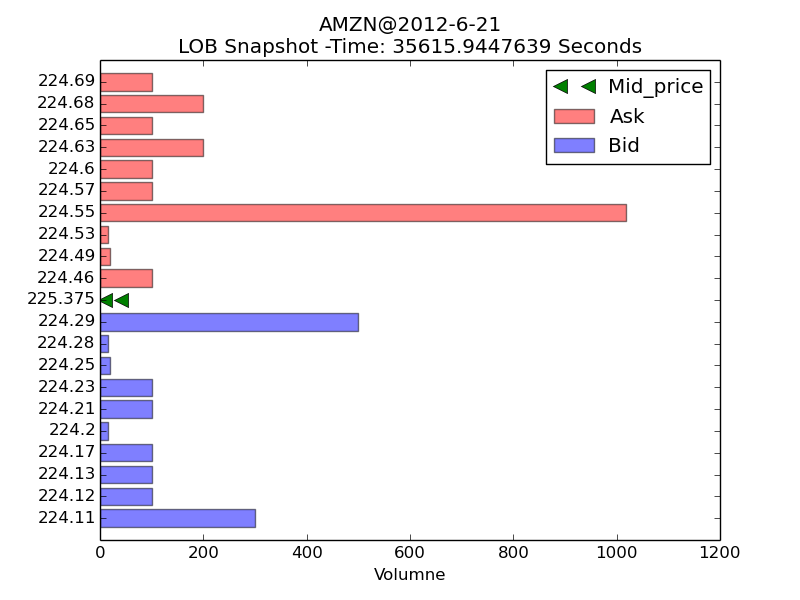
\includegraphics[width=1\textwidth, height=0.6\textheight]{orderbook_example.png}
			\end{center}
		\end{column}
		\begin{column}{.5\textwidth}
			\begin{itemize}
			\item At Time t: $P_t^A>P_t^B$, no arbitrage 
			\item At Time t+ $\Delta t$, there are three situations:\\
			\subitem \textbullet $P_{t+\Delta t}^A<P_t^B$: \alert{ask lower},denote as 1 in our model
			\\
			\subitem\textbullet  $P_{t+\Delta t}^B>P_t^A$: \alert{bid higher}, denote as -1 in our model
			\\
			\subitem\textbullet  otherwise(implies that \alert{no direction} change)
			\end{itemize}
		\end{column}
	\end{columns}
	\hover<2>{
	      \begin{minipage}{0.8\linewidth}
	        \begin{block}{Our major concern is:}
	        \alert{Cross over opportunities}, that is bid higher or ask lower after some time.
	        \end{block}
	      \end{minipage}
	      }	
\end{frame}


\begin{frame}
\frametitle{Model fit}
\textbf{Ask low example(5 seconds future):}
\begin{figure}
\centering
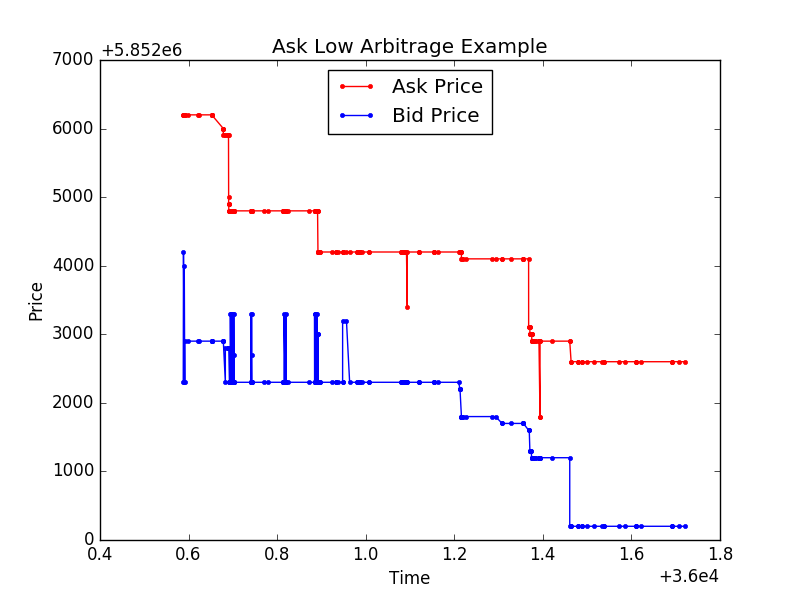
\includegraphics[width=0.7\linewidth]{./ask_low_example}
\caption{Ask low arbitrage example}
\label{fig:ask_low_example}
\end{figure}

\end{frame}

\begin{frame}

\textbf{Bid high example(5 seconds future):}
\begin{figure}
\centering
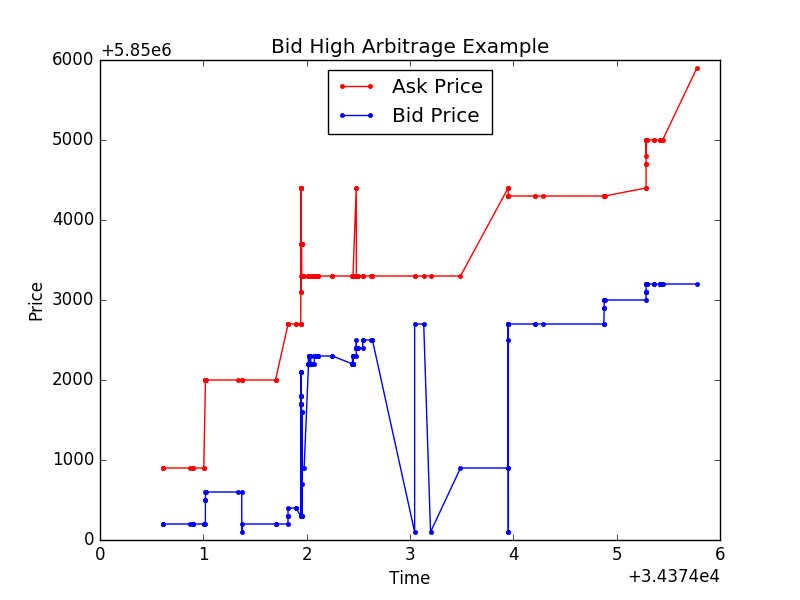
\includegraphics[width=0.7\linewidth]{./bid_high_example}
\caption{Bid high arbitrage example}
\label{fig:bid_low_example}
\end{figure}

\end{frame}


\begin{frame}
\frametitle{Model fit}
\textbf{No arbitrage example(5 seconds future):}
\begin{figure}
\centering
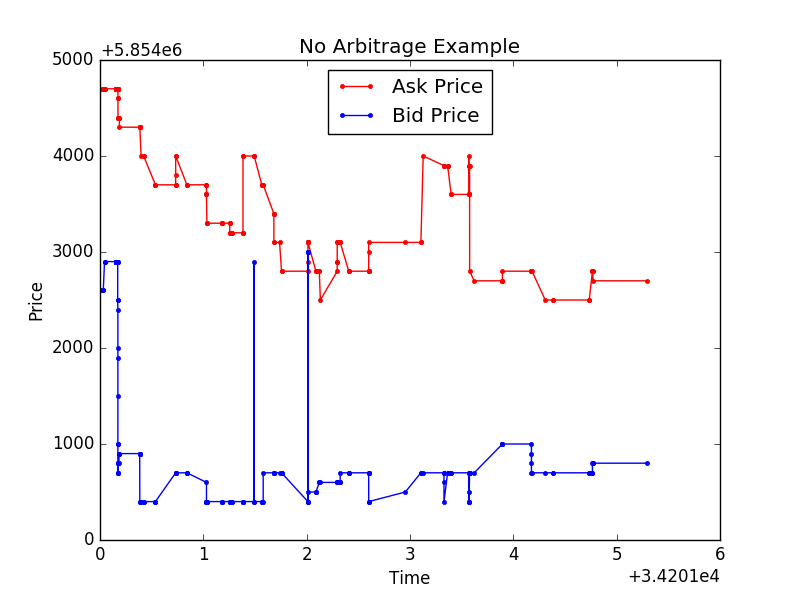
\includegraphics[width=0.7\linewidth]{./no_arbi_example}
\caption{No arbitrage example}
\label{fig:no_arbi_example}
\end{figure}

\end{frame}

\begin{frame}
\frametitle{Stock Price}
\begin{columns}		
		\begin{column}{.5\textwidth}
		   \textbf{AAPL:}

						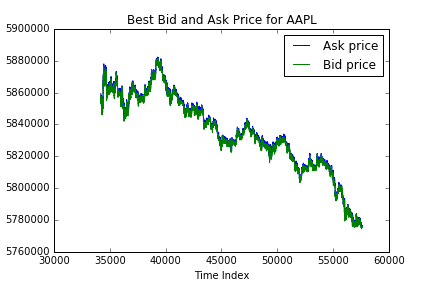
\includegraphics[width=1\textwidth, height=0.4\textheight]{AAPL_price.png}

			 \textbf{AMZN:}

									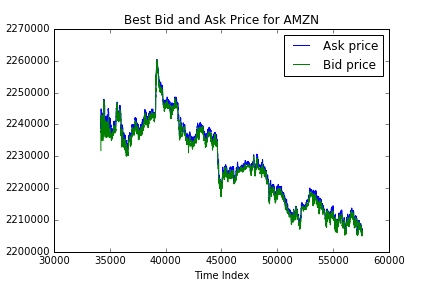
\includegraphics[width=1\textwidth, height=0.4\textheight]{AMZN_price.png}

		\end{column}
		\begin{column}{.5\textwidth}
			 \textbf{GOOG:}

									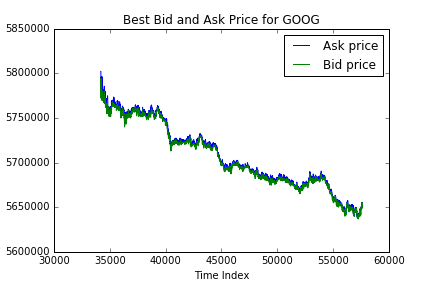
\includegraphics[width=1\textwidth, height=0.4\textheight]{GOOG_price.png}

			 \textbf{INTC:}
	
										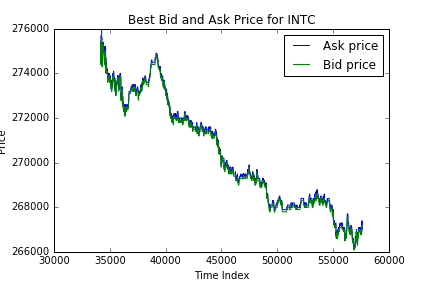
\includegraphics[width=1\textwidth, height=0.4\textheight]{INTC_price.png}

		\end{column}
	\end{columns}

\end{frame}




\begin{frame}
\frametitle{Model fit}
\textbf{Arbitrage opportunities based on future event}
\begin{columns}		
		\begin{column}{.5\textwidth}
		   \textbf{AAPL:}

						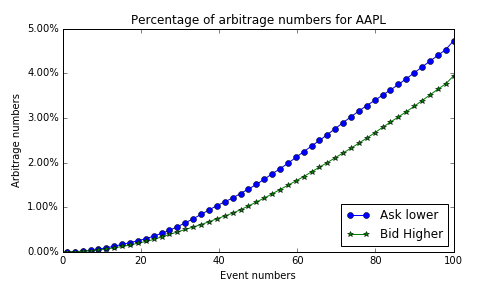
\includegraphics[width=1\textwidth, height=0.4\textheight]{AAPL_arbitrage_event.png}

			 \textbf{AMZN:}

									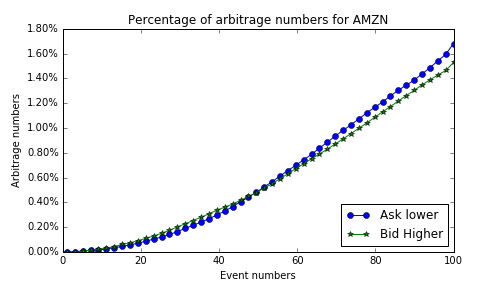
\includegraphics[width=1\textwidth, height=0.4\textheight]{AMZN_arbitrage_event.png}

		\end{column}
		\begin{column}{.5\textwidth}
			 \textbf{GOOG:}

									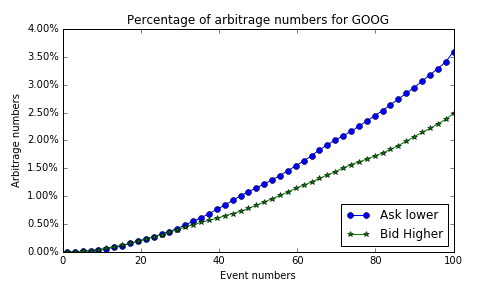
\includegraphics[width=1\textwidth, height=0.4\textheight]{GOOG_arbitrage_event.png}

			 \textbf{INTC:}
	
										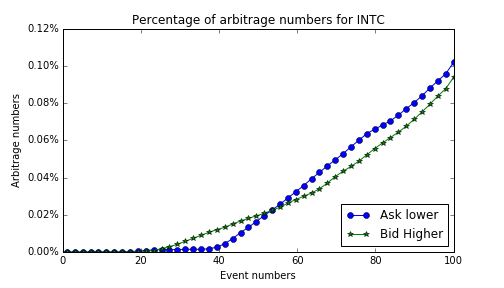
\includegraphics[width=1\textwidth, height=0.4\textheight]{INTC_arbitrage_event.png}

		\end{column}
	\end{columns}

\end{frame}



\begin{frame}
\frametitle{Model fit}
\textbf{Arbitrage opportunities based on future time}
\begin{columns}		
		\begin{column}{.5\textwidth}
		   \textbf{AAPL:}

						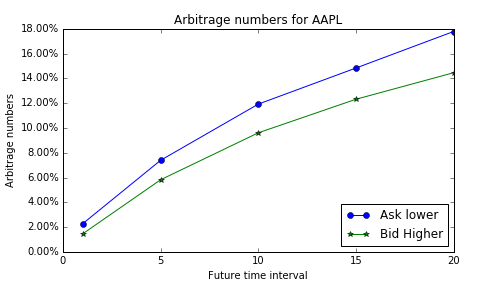
\includegraphics[width=1\textwidth, height=0.4\textheight]{AAPL_arbitrage_time.png}

			 \textbf{AMZN:}

									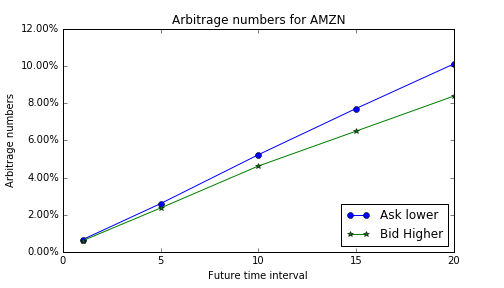
\includegraphics[width=1\textwidth, height=0.4\textheight]{AMZN_arbitrage_time.png}

		\end{column}
		\begin{column}{.5\textwidth}
			 \textbf{GOOG:}

									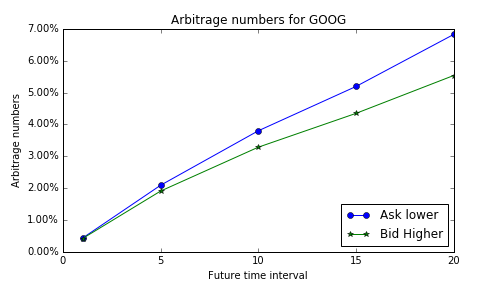
\includegraphics[width=1\textwidth, height=0.4\textheight]{GOOG_arbitrage_time.png}

			 \textbf{INTC:}
	
										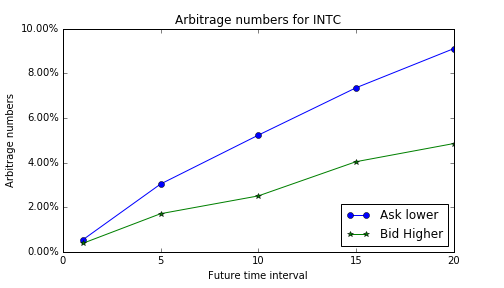
\includegraphics[width=1\textwidth, height=0.4\textheight]{INTC_arbitrage_time.png}

		\end{column}
	\end{columns}

\end{frame}



\begin{frame}
\frametitle{Model fit}
\textbf{Order book type}

\begin{center}	
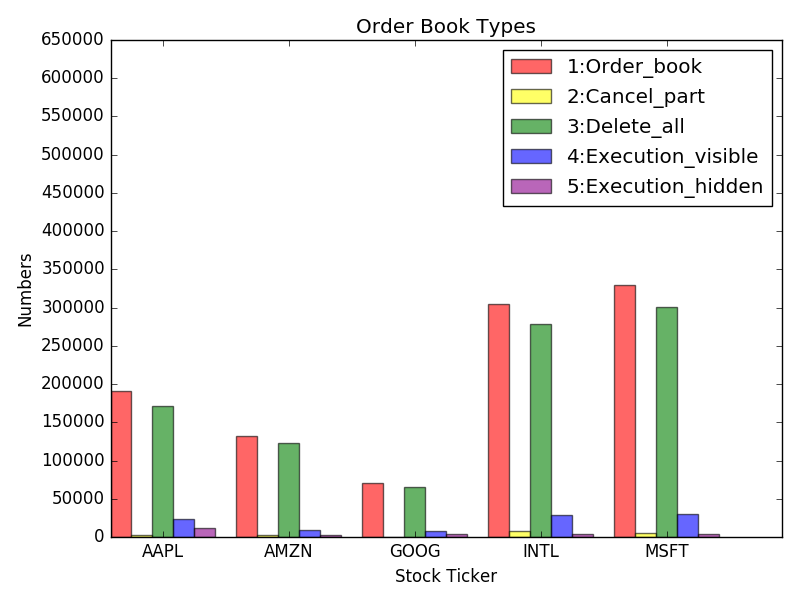
\includegraphics[width=1\textwidth, height=0.7\textheight]{order_book_type.png}
\end{center}
\textbf{Red and green occupy the most, momentum ignition?}
\end{frame}


\begin{frame}
\frametitle{Model fit}
\textbf{Order book volume}

\begin{center}	
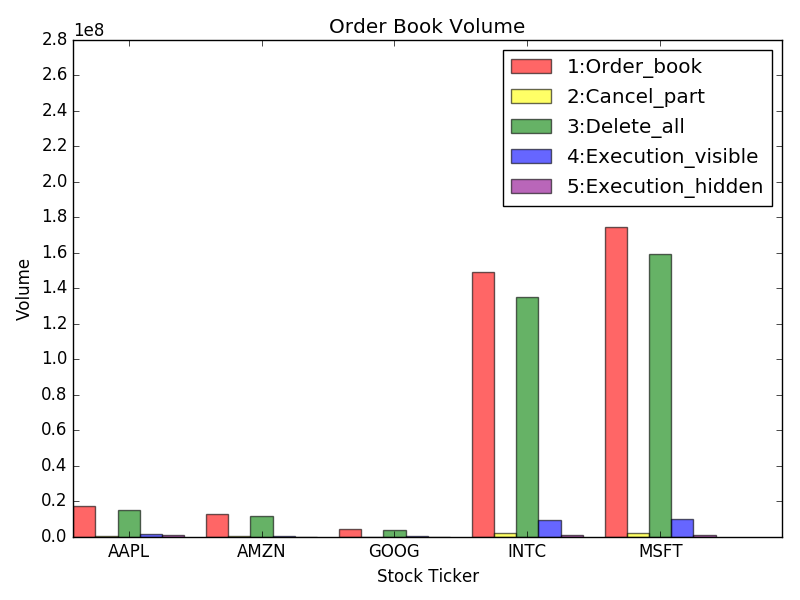
\includegraphics[width=1\textwidth, height=0.7\textheight]{order_book_volume.png}
\end{center}
\textbf{Still red and green occupy the most}
\end{frame}


\begin{frame}
\frametitle{Model fit}
\textbf{Build features:}\\
We use same features that presented by Dr.Kercheval and Yuan Zhang(2015)
	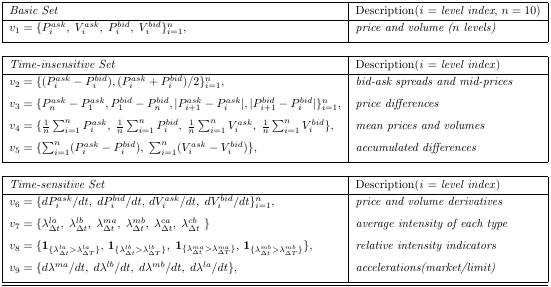
\includegraphics[width=1\textwidth, height=0.6\textheight]{features.png}
\begin{itemize}\footnotesize
			\item contain \alert{price,volume, bid ask spread, price difference and volume difference for each level, mean of price and volume.}  
            \item total 138 variables,  can be treated as high dimensional problems.
\end{itemize}
\end{frame}


\begin{frame}
\frametitle{Model fit}
\small \textbf{Criteria: Only consider accuaracy? Imbalanced data? Pay more attention to rare events}\\
\begin{block}{Precision}
\scriptsize{Precision is the probability that a (randomly selected) detected arbitrage opportunties is real arbitrage opportunites.}\\
\center{
$Precision=\frac{True\_positive}{True\_positive + False\_positive}$
}
\end{block}
\begin{block}{Recall}
\scriptsize{Recall is the probability that a (randomly selected) real arbitrage opportunity is detected by our model.}\\
\center{
$Recall=\frac{True\_positive}{True\_positive + False\_negative}$
}
\end{block}
\begin{block}{F1 score}
\scriptsize{A measure that combines precision and recall is the harmonic mean of precision and recall.}\\
\center{
$F_\beta=(1+\beta^2)  \frac{precision\cdot recall}{\beta^2  precision+recall}$
}
\end{block}

\end{frame}


\begin{frame}
\frametitle{Methodology}
\textbf{Data sample stability:}
Changing data sample size, see the influence to the f1 score. Can use intra-data to predict. Use AAPL and AMZN as exampels:\\

\begin{center}
     \includegraphics[width=1\textwidth, height=0.45\textheight]{data_stability.png}
\end{center}

F1 score did not always increase when the data sample size increased. So may use relative small size data to train the model.

\end{frame}
\begin{frame}
\frametitle{Numerical results:}

\begin{block}{AMZN ask low predict(5 seconds):}
\textbk{train to test ratio is: 9:1}
\begin{table}[h!]\scriptsize
  \caption{AAPL Accuracy rate and CPU time}
\begin{center}
    \begin{tabular}{| c | c|c|c|c|}
    \hline

Model&	Training &	Training &	Test &	Test\\
&	time(s)&	accuracy&	accuracy&	f1 score\\
    \hline
Logistic(Lasso penalty)&	538&	97.71\%& 	98.45\%& 	8.28\%\\
Logistic(Ridge penalty)	& 7&	97.71\%& 	98.45\%& 	8.28\%\\
SVM(Poly 2 kernal,5000 estimator)&  	72& 	98.70\%& 	99.00\%&	54.95\%\\
Decision Tree(no maximum depth)&	3.76& 	98.67\%& 	98.95\%& 	51.61\% \\
Ada boosting(100 estimator)&	365& 	99.99\%& 	99.02\%& 	\alert{79.32}\%\\
Random forest( 100 estimator)&	31& 	99.80\%& 	99.15\%& 	\alert{80.91}\%\\


\hline
\end{tabular}
\end{center}
\end{table}
\end{block}
\small{remark: \alert{training samples 90000 and test samples 10000}. The estimation number for AdaBoost and random forest is 100.Computer is 8G memory and Intel Xeon E3 processor(4 cores)}
\end{frame}​






\begin{frame}
\frametitle{Methodology}
\textbf{Classification matrix for multi-class classification results:ask low as 1 and bid high as -1}\\
\begin{columns}
\column{2.3in}
	\begin{block}{One against One}
\begin{equation*}       
\left[           
  \begin{array}{ccc}   
    172&    54 &    0\\  
     1& 9416& 4\\  
    0  &  153 & 200
  \end{array}
\right]               
\end{equation*}
\begin{center}
     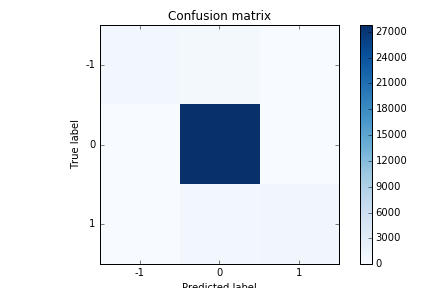
\includegraphics[width=1\textwidth, height=0.45\textheight]{one_vs_one.png}
\end{center}
\end{block}
\column{2.3in}

	\begin{block}{One against Rest}
\begin{equation*}       
\left[           
  \begin{array}{ccc}   
    166&    60 &    0\\  
     1& 9416& 4\\  
    0  & 150 & 203
  \end{array}
\right]               
\end{equation*}
\begin{center}
     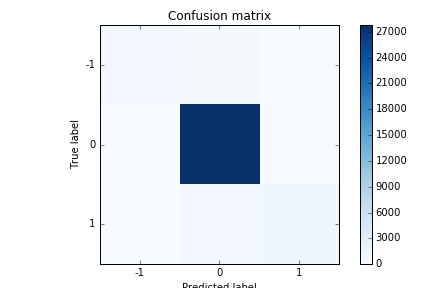
\includegraphics[width=1\textwidth, height=0.45\textheight]{one_vs_rest.png}
\end{center}     
\end{block}
\end{columns}

\end{frame}


\section{Trading strategy and PnL results}

\begin{frame}
\frametitle{PnL}
According to Nan Zhou, Wen Cheng, Yichen Qin & Zongcheng Yin(2015) in quantitative finance.

PnL is the profit and loss through transaction, formula of PnL can be written as follows:\\
\begin{equation*}       
PnL=\left\{          
  \begin{array}{ll}   
    y-c  & y>=\alpha, buy\ action   \\  
     -y-c & y<=-\alpha, sell\ short\ action \\
     0 & otherwise
  \end{array}
\right.       
\end{equation*}

where y is the net capital gain from transaction, $\alpha$ is significant level and $c$ is trading cost.
\end{frame}



\begin{frame}
\frametitle{Trading strategy}
		\textbf{Naive trading strategy:}\\
Assume: $\alpha$ and $c$ equal to 0
		\begin{algorithm}[H]
				         		    \dontprintsemicolon
				         		    \linesnumbered
				         		    \nl initialize: PnL=0\\				         		    
				         		    \nl \For{i =1 to length(test\_set)}{
				         		    \nl input test\_set[i] features into model and get result of Predict[i]\\
				         		    \nl \If{Predict[i]==1(Ask low)}{
				         		         Sell short at bid price\\
				         		         Clear the short option $\Delta t$ seconds later\\
				         		         PnL+=$Bid\_price_{t}-Ask\_price_{t+\Delta t}$}
				         		        \ElseIf{Predicted[i]==-1(Bid high)}
				         		         {Buy at ask price\\
				         		         Sell at bid price $\Delta t$ seconds later\\
				         		          PnL+=$Bid\_price_{t+\Delta t}-Ask\_price_t$}\\
				         		        \Else
				         		         {Take no action} \\
				         		    \nl  \Return PnL 
				         		     }				         		    				         		    
				         		    
			\end{algorithm} \\

\end{frame}

\begin{frame}
\textbf{Strategy framework:}
\begin{center}
     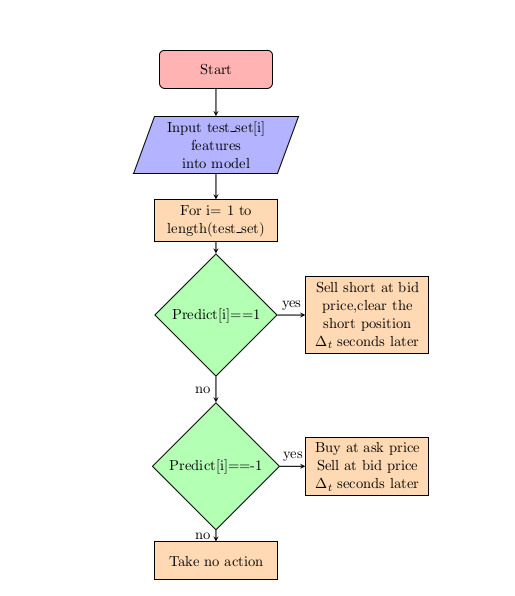
\includegraphics[width=0.8\textwidth, height=0.9\textheight]{strategy_algorithm.png}
\end{center}    
\end{frame}

\begin{frame}
\frametitle{Trading strategies:}


\begin{center}
     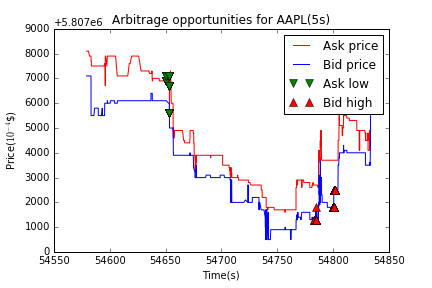
\includegraphics[width=0.6\textwidth, height=0.6\textheight]{arbitrage_plot.png}
\end{center}    
Ask low occurs: sell short current bid price. Bid high occurs: buy at current ask price
\end{frame}


\begin{frame}
\frametitle{Each PnL result:}
\textbf{one against rest example:}\\
For simplicity, assume both significant level $\alpha$ and trading cost $c$ equal to 0.
\begin{center}
     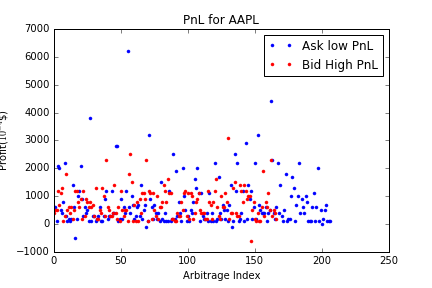
\includegraphics[width=0.6\textwidth, height=0.6\textheight]{AAPL_pnl.png}
\end{center}    

\end{frame}


\section{Future work}
\begin{frame}
\frametitle{Future work}
    \begin{itemize}
        \item  Compare the results in spark machine learning package.Can deal with big data problem 
        \item  Add more meaningful features and calculate the interaction.
        \item  Neural network and deep learning.  AlphaGo Google deepmind?
        \item  Submit on journal of high frequency or quantitative finance 
      \end{itemize}
\end{frame}

\begin{frame}
\begin{block}{Reference}
 \begin{thebibliography}{1}\itemsep=-0.4em
      \setlength{\baselineskip}{0.2em}
     
           \bibitem{alec:model}
             Alec N.Kercheval,Yuan Zhang        
             \newblock Modeling high-frequency limit order book dynamics
             with support vector machines        
             \newblock In {\em Quantitative finance 2014}
     
      \bibitem{rosu:dynamic}
      Rosu,I., 
      \newblock A dynamic model of the limit order book. 
      \newblock In {\em Rev.Financ.Stud.,2009,22,4601-4641.}
      
        \bibitem{:recognition}
                Trevor Hastie, Robert Tibshirani, Jerome Friedman      
                \newblock The Elements of Statistical Learning: Data Mining, Inference, and Prediction,Second Edition        
               
      \end{thebibliography}
\end{block}
\end{frame}

\section{Questions}

\begin{frame}
\frametitle{QA}
\begin{center}
\huge{Thanks a lot and Questions}
\end{center}
\end{frame}

\end{document}

